\chapter{Testing \& Evaluation}
\label{chapter6}

The testing process was made of two steps. First, an efficiency evaluation of the package was made to determine the computational time needed for the whole logic to run. Finally, each individual component in the package was separately tested in indoor environments, where such an interface could be made use of.

\section{Timing breakdowns}

Efficiency was an important attribute to the project since the early planning stage, as the solution is targeted towards real-time applications usage. In this section the timing measurements for each module are presented along with a small discussion about the average execution time and whether the original target was reached.

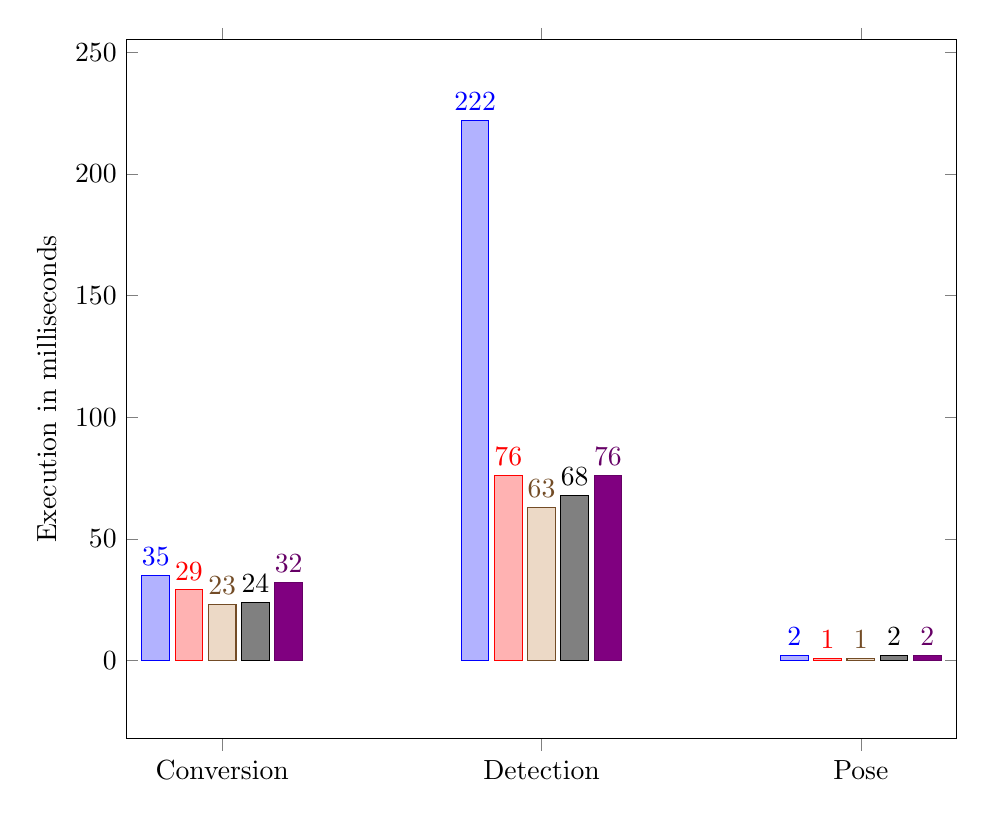
\begin{tikzpicture}
	\begin{axis}[
    	ybar,
        enlargelimits=0.15,
        legend style={at={(0.5,-0.15)},
        anchor=north,legend columns=-1},
        ylabel={Execution in milliseconds},
        symbolic x coords={Conversion, Detection, Pose},
        xtick=data,
        nodes near coords,
        nodes near coords align={vertical},
        width=\textwidth
        ]
        \addplot coordinates {(Conversion, 35) (Detection, 222) (Pose, 2)};
        \addplot coordinates {(Conversion, 29) (Detection, 76) (Pose, 1)};
        \addplot coordinates {(Conversion, 23) (Detection, 63) (Pose, 1)};
        \addplot coordinates {(Conversion, 24) (Detection, 68) (Pose, 2)};
        \addplot coordinates {(Conversion, 32) (Detection, 76) (Pose, 2)};
	\end{axis}
\end{tikzpicture}

From the histogram of the time breakdowns showed above, all of the modules do perform extremely efficiently. In particular, the conversion component takes on average \textbf{28.6 milliseconds} to finish the conversion step. Detecting people on the RGB frame, which is by far the most computationally expensive step, takes an average of only \textbf{101 milliseconds}. Finally, the 3D pose estimation module was unsurprisingly the fastest one, as it completes the computation in only \textbf{1.6 milliseconds}.

The average computational time for the package to carry out the estimation process is of only \textbf{43.7 milliseconds}. Therefore, the original objective of developing a ROS package usable in real-time can be considered met.

\section{Module Testing}

In this section the testing is primarily focused on the individual modules. In particular, the detection and pose module are tested in isolation to check their performance within indoor environments. Note that the conversion module is not tested as it does not have a real impact in the ultimate estimation.

\subsection{Person Detection}

The detection's module tests were carried in two different environments, one being the robotics lab at the University of Leeds whose lighting conditions are not the best and whose space is really crammed and cluttered with objects, and the long-room area which offers a sparse area with a good lighting conditions. Clutter, occlusions, scale and lighting conditions were the situations tested.

\subsubsection{Light conditions, Scale \& Clutter}

\begin{figure}[H]
    \begin{subfigure}{.5\textwidth}
        \centering
        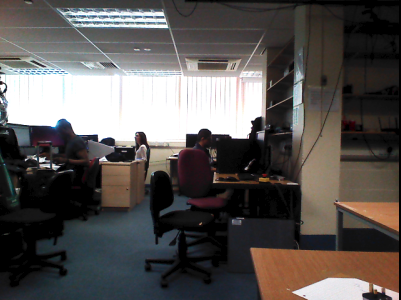
\includegraphics[width=.9\linewidth]{images/chapter6_clutter_light.png}
        \caption{Poor light condition and clutter.}
	\end{subfigure}
    \begin{subfigure}{.5\textwidth}
        \centering
        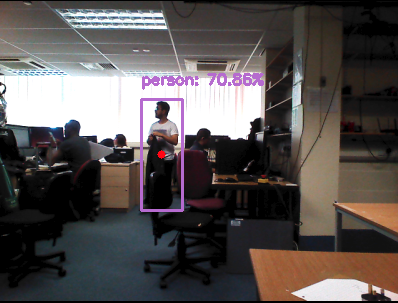
\includegraphics[width=.9\linewidth]{images/chapter6_clutter_light_detection.png}
        \caption{Detection in clutter.}
	\end{subfigure}
    \begin{subfigure}{.5\textwidth}
        \centering
        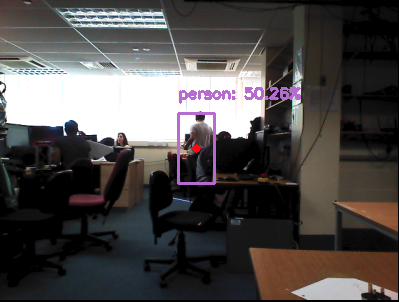
\includegraphics[width=.9\linewidth]{images/chapter6_clutter_light_detection_back.png}
        \caption{Detection in clutter (person showing back).}
	\end{subfigure}
    \begin{subfigure}{.5\textwidth}
        \centering
        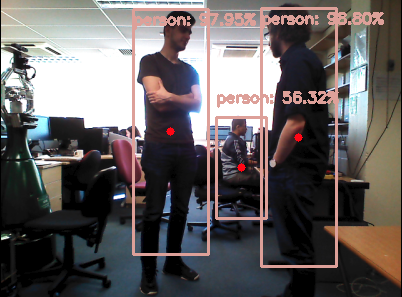
\includegraphics[width=.9\linewidth]{images/chapter6_clutter_standing.png}
        \caption{Multiple detections in clutter.}
	\end{subfigure}
\end{figure}

The outcomes of the detection module in poor lighting conditions are variable. In fact, Figure (a) shows a poor performance in the detection process as none of the three subjects in the picture were detected. However, this is not entirely to be attributed to the lighting conditions as the individuals are all partially occluded in the clutter of the lab.

Figure (b) and (c) show an improvement in the detection outcome when one of the individuals is standing in the room. Both situations present a difficult situation, as in (b) the subject has his lower-body covered by a jacket and in (c) the same person is standing showing only his back and still partially covered which determines the low confidence in the detection, which is only 50\%.

Figure (d) shows a robust detection result when the subjects are standing clearly even in poor lighting conditions and when not facing directly the camera. Moreover, the same figure shows how well the module handles detections at different scales by detecting a third seated person further down the room.

\subsubsection{Occlusions}

\begin{figure}[H]
    \begin{subfigure}{.5\textwidth}
        \centering
        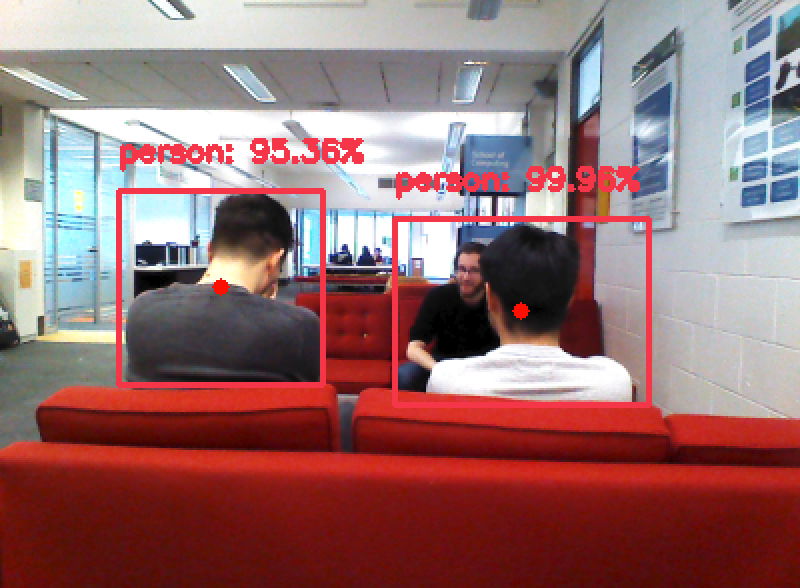
\includegraphics[width=.9\linewidth]{images/chapter6_occlusion_seated.png}
        \caption{Occlusion due to overlapping.}
	\end{subfigure}
    \begin{subfigure}{.5\textwidth}
        \centering
        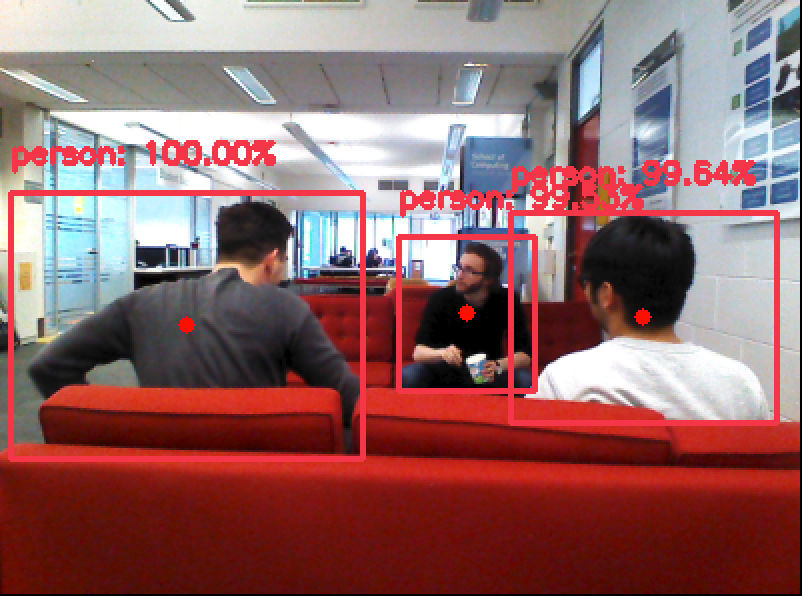
\includegraphics[width=.9\linewidth]{images/chapter6_occlusion_seated_good.png}
        \caption{Correct detection in occlusion.}
	\end{subfigure}
    \begin{subfigure}{.5\textwidth}
        \centering
        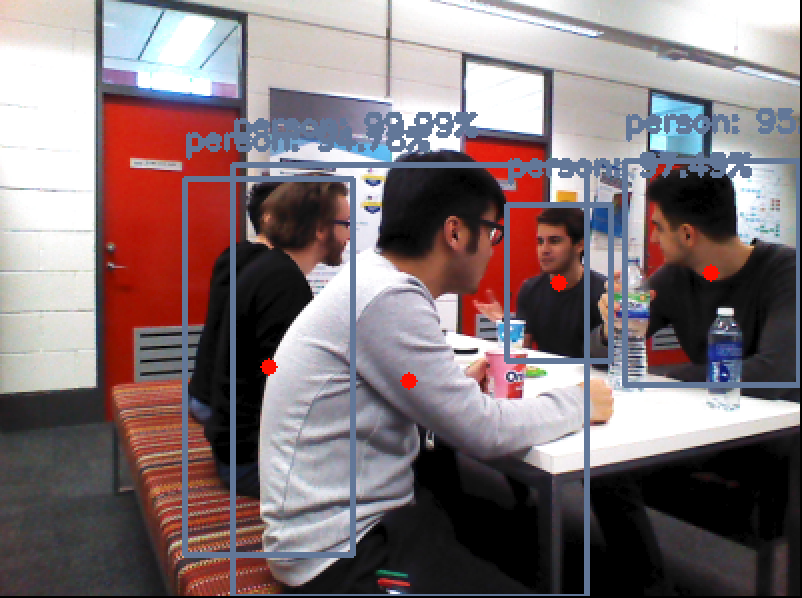
\includegraphics[width=.9\linewidth]{images/chapter6_occlusion_table_back.png}
        \caption{Seated occlusion.}
	\end{subfigure}
    \begin{subfigure}{.5\textwidth}
        \centering
        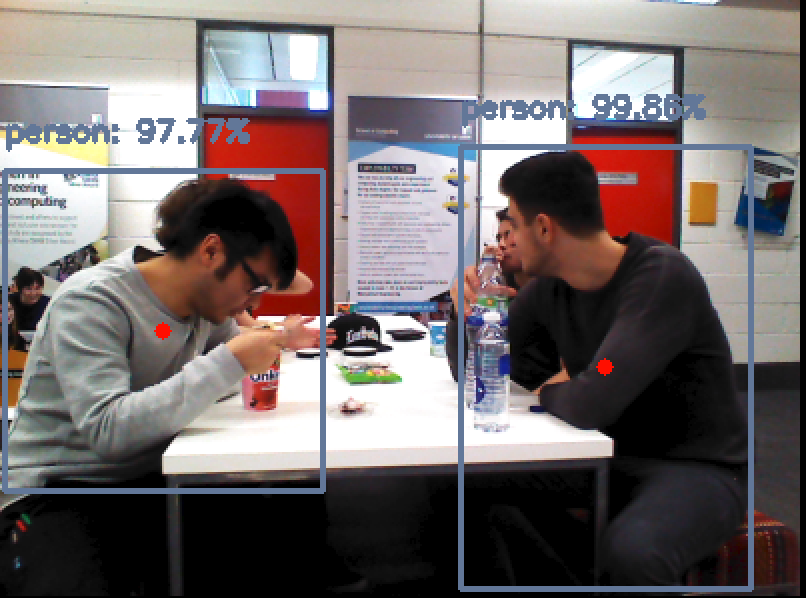
\includegraphics[width=.9\linewidth]{images/chapter6_occlusion_table_side.png}
        \caption{Sideway occlusion.}
	\end{subfigure}
\end{figure}

In Figure (a) the neural network fails at separating between the two subjects sitting to the right of the sofa, although the distinction is clearly visible. Figure (b) shows a good detection result when the occluding person moves to the right. Finally, we notice how in both (a) and (b) the two people sitting with their back towards the camera where detected even though only a part of their upper-back was showing, with an incredible 100\% confidence for one of the subjects in (b).

In Figure (c) the module is able to detect four out of the five participants, in a situation where three of these are either occluded by the table or other subjects. In (d) the same scenario as (c) is presented but from a side perspective. In this occasion only two people at the for-front are being detected as the remaining three subjects are completely or majority occluded by these.

\subsubsection{Final Conclusion}

The module can be considered to be highly reliable given its correctness in detecting people in all sorts of positions and variables, as well as its robustness against false positives instances as throughout the testing not once a non-person was detected as such.

\subsection{Pose Estimation}

To test the distance and 3D pose computations three different scenarios were carried out in the robotics lab. For each scenario the correct 3D pose of each individual was noted down along using the point cloud data in RVIZ. The measurement is then used as a comparison to the estimated 3D pose of the package. The red markers in the RVIZ images below show the estimated position while the violet ones the actual one.

\subsubsection{Scenario1}

\begin{figure}[H]
    \begin{subfigure}{.5\textwidth}
        \centering
        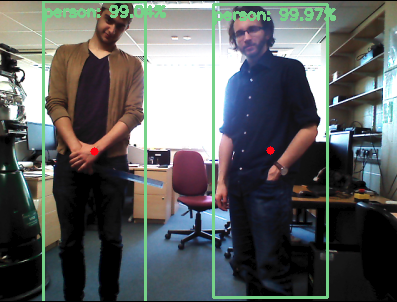
\includegraphics[width=\linewidth]{images/chapter6_scenario1.png}
        \caption{Scenario1 frame.}
        \label{2a}
	\end{subfigure}
    \begin{subfigure}{.5\textwidth}
        \centering
        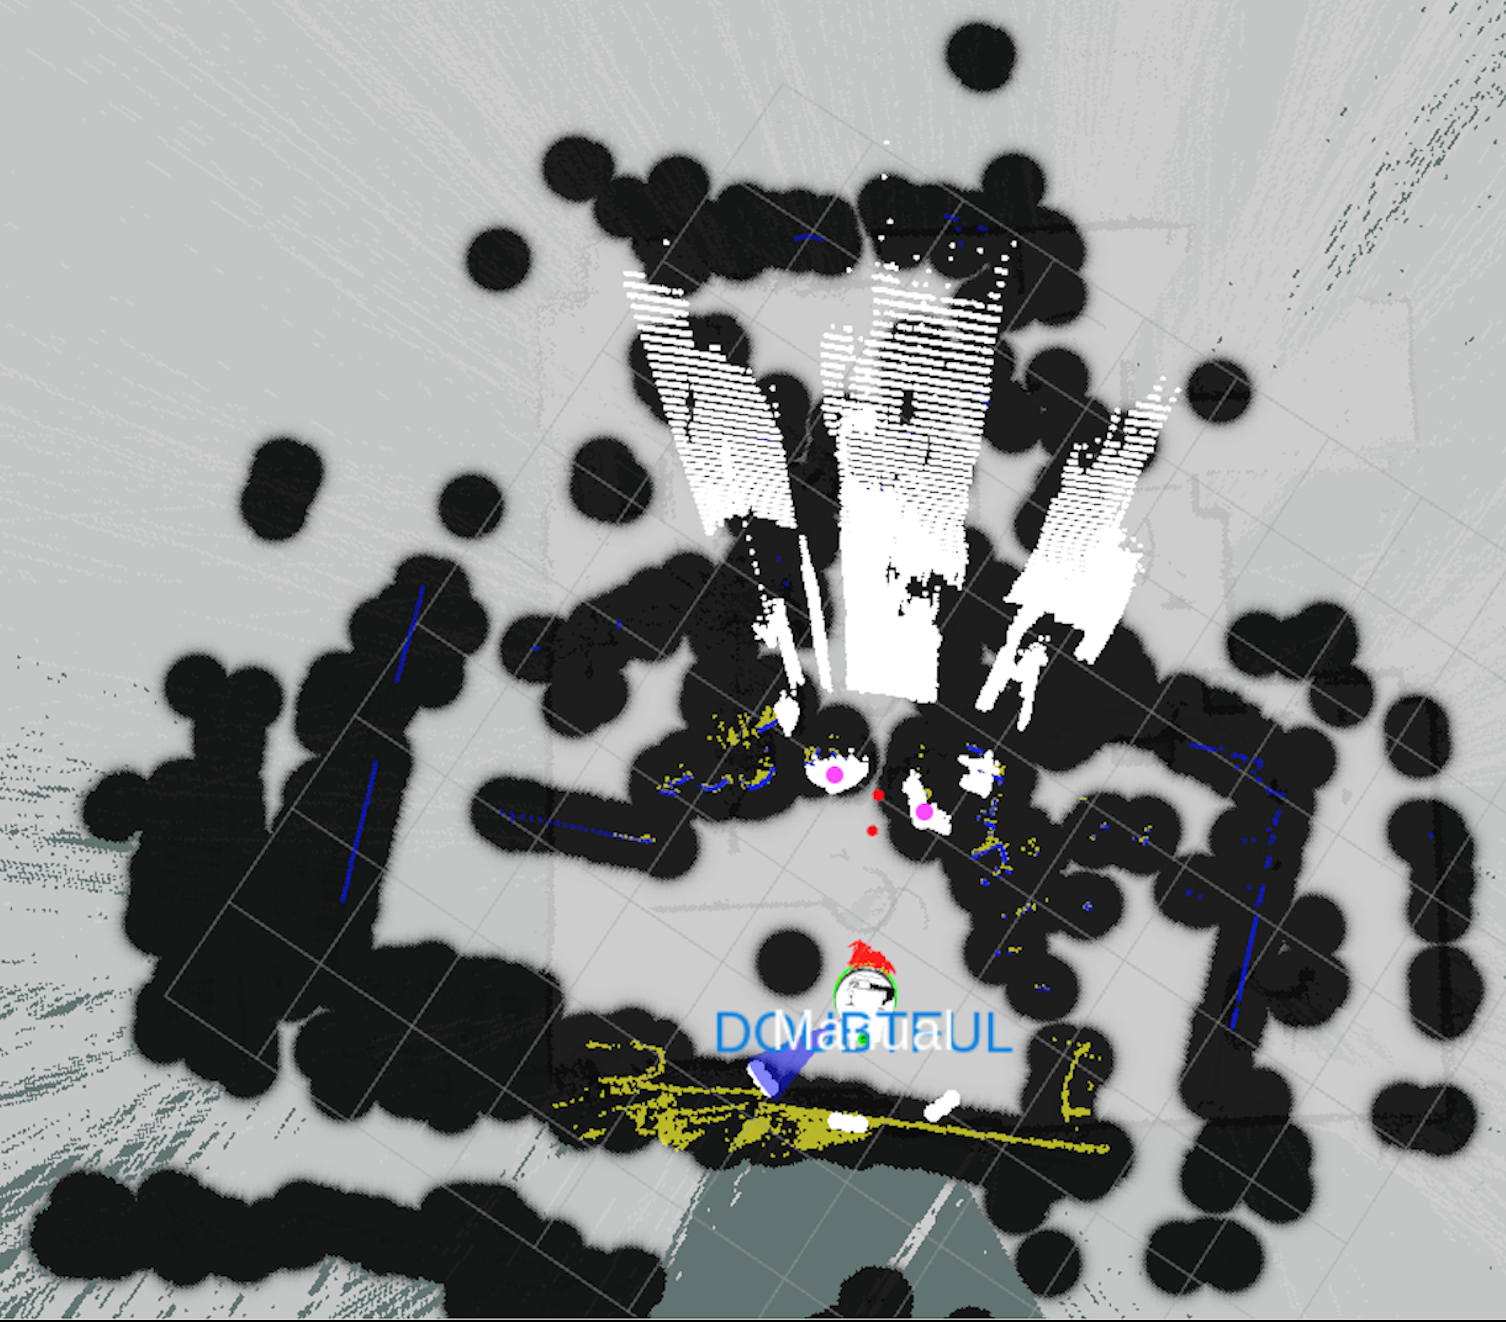
\includegraphics[width=\linewidth]{images/chapter6_rviz_extend.png}
        \caption{Scenario1 markers.}
        \label{2b}
	\end{subfigure}
\end{figure}

\begin{table}[H]
  \centering
  \begin{tabular}{ |p{4cm}|p{2cm}|p{2cm}|p{2cm}|  }
    \hline
    \multicolumn{4}{|c|}{Scenario1: 3D Pose Data} \\
    \hline
    & \textbf{X} & \textbf{Y} & \textbf{Z} \\
    \hline
    Real (Left) & 0.856 & 0.633 & 0.00293 \\
    Estimated (Left) & 0.738 & 0.519 & 0.00203 \\
    \hline
    Real (Right) & 0.0497 & 0.264 & 0.00149 \\
    Estimated (Right) & 0.0623 & 0.192 & 0.00475 \\
    \hline
  \end{tabular}
\end{table}



\subsubsection{Scenario2}

\begin{figure}[H]
    \begin{subfigure}{.5\textwidth}
        \centering
        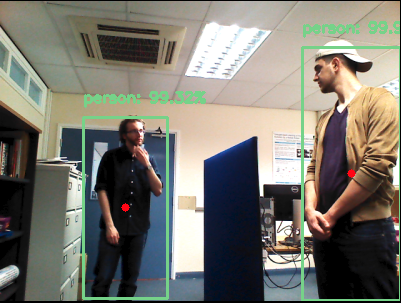
\includegraphics[width=8cm]{images/chapter6_scenario2.png}
        \caption{Scenario1 frame.}
        \label{2a}
	\end{subfigure}
    \begin{subfigure}{.5\textwidth}
        \centering
        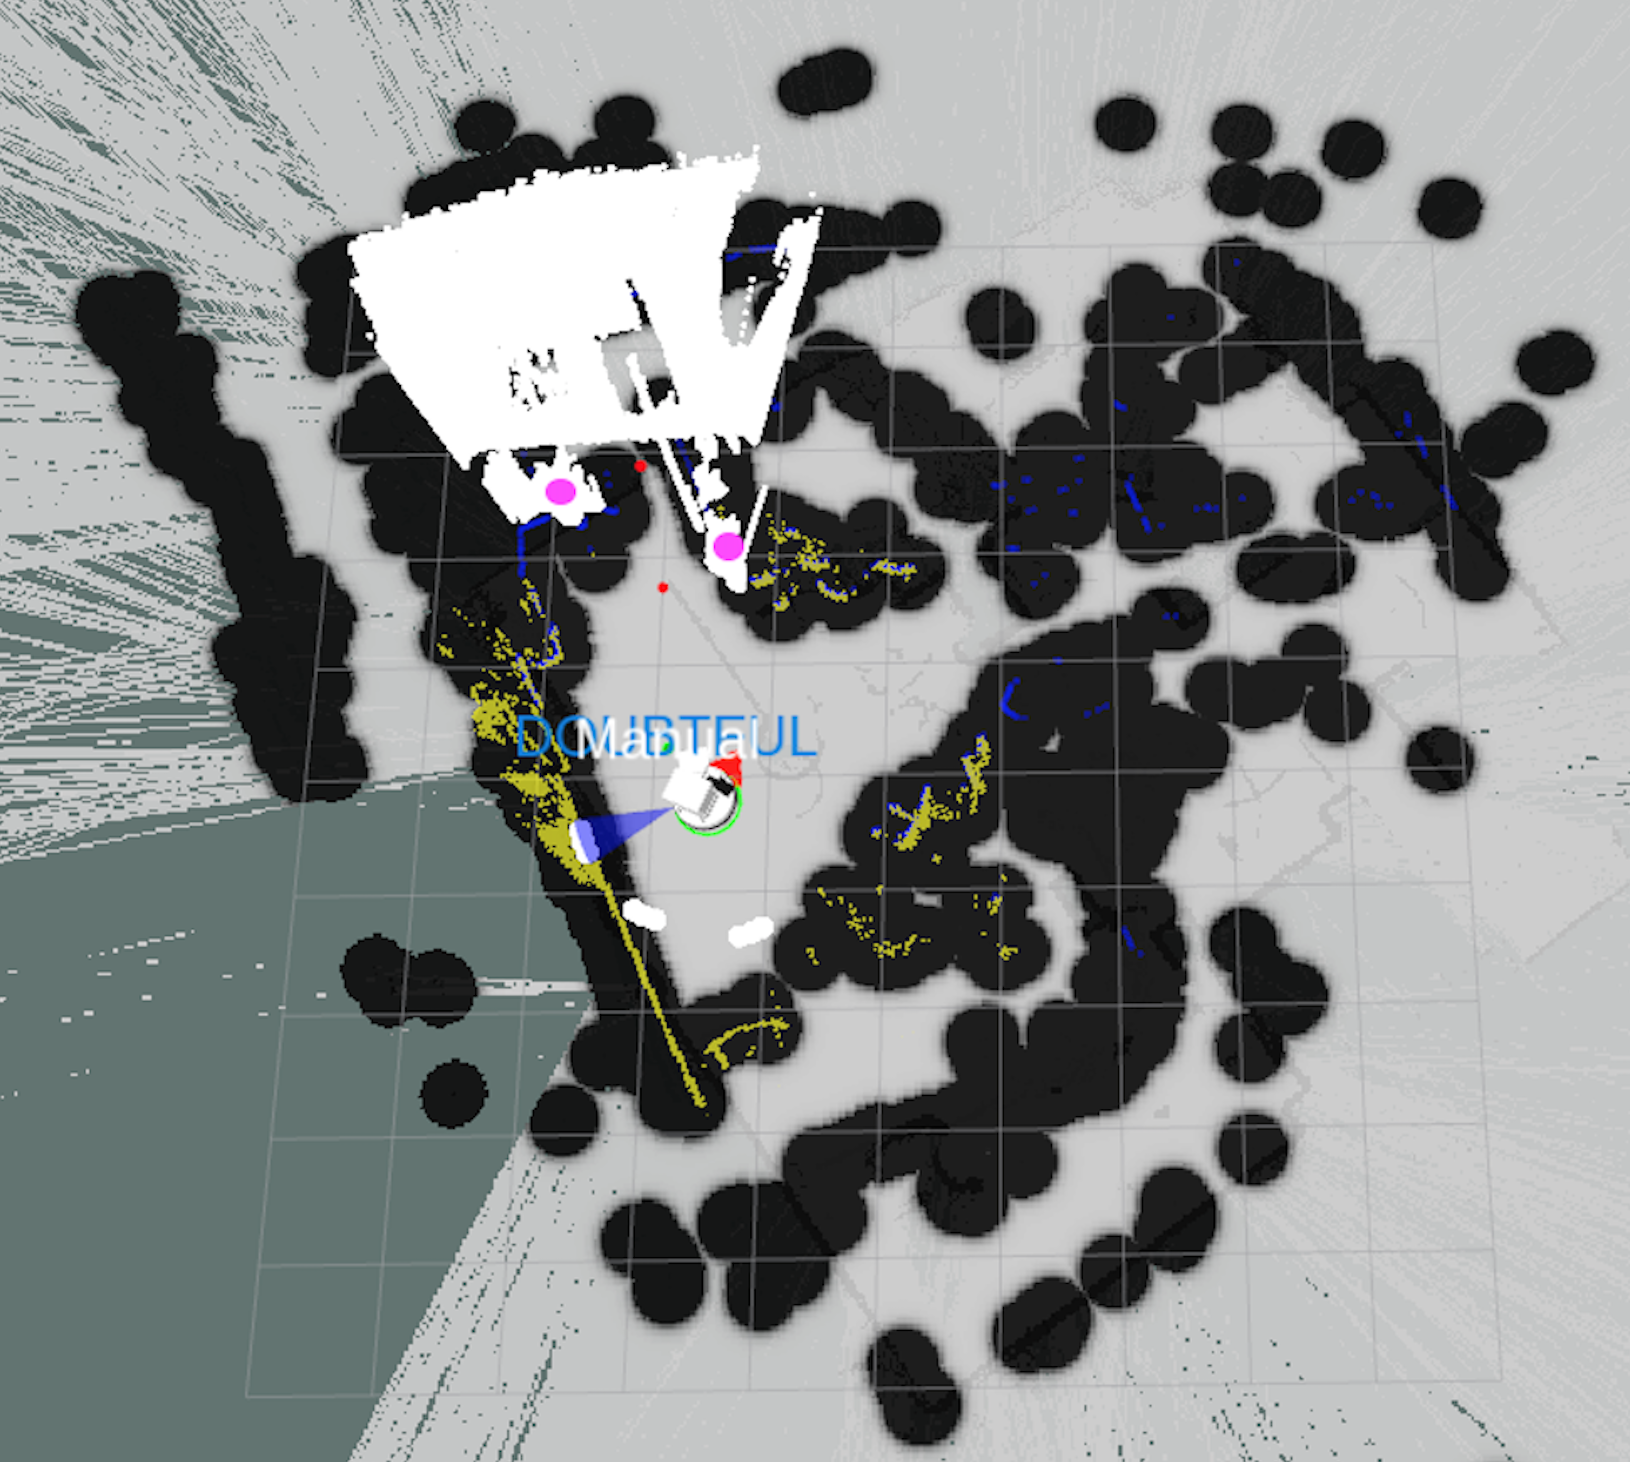
\includegraphics[width=.9\linewidth]{images/chapter6_rviz_extend2.png}
        \caption{Scenario1 markers.}
        \label{2b}
	\end{subfigure}
\end{figure}

\begin{table}[H]
  \centering
  \begin{tabular}{ |p{4cm}|p{2cm}|p{2cm}|p{2cm}|  }
    \hline
    \multicolumn{4}{|c|}{Scenario1: 3D Pose Data} \\
    \hline
    & \textbf{X} & \textbf{Y} & \textbf{Z} \\
    \hline
    Real (Left) & 2.17 & 2.61 & 0.00248 \\
    Estimated (Left) & 2.63 & 2.11 & 0.00357 \\
    \hline
    Real (Right) & 1.73 & 1.11 & 0.00547 \\
    Estimated (Right) & 1.4 & 1.67 & 0.00666 \\
    \hline
  \end{tabular}
\end{table}
\clearpage

\subsubsection{Scenario3}

\begin{figure}[H]
    \begin{subfigure}{.5\textwidth}
        \centering
        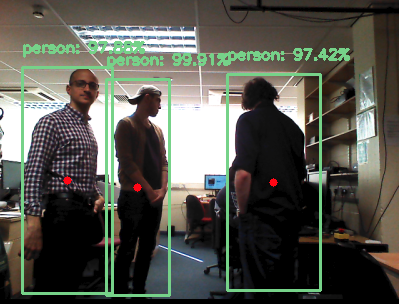
\includegraphics[width=8cm]{images/chapter6_scenario3.png}
        \caption{Scenario1 frame.}
        \label{2a}
	\end{subfigure}
    \begin{subfigure}{.5\textwidth}
        \centering
        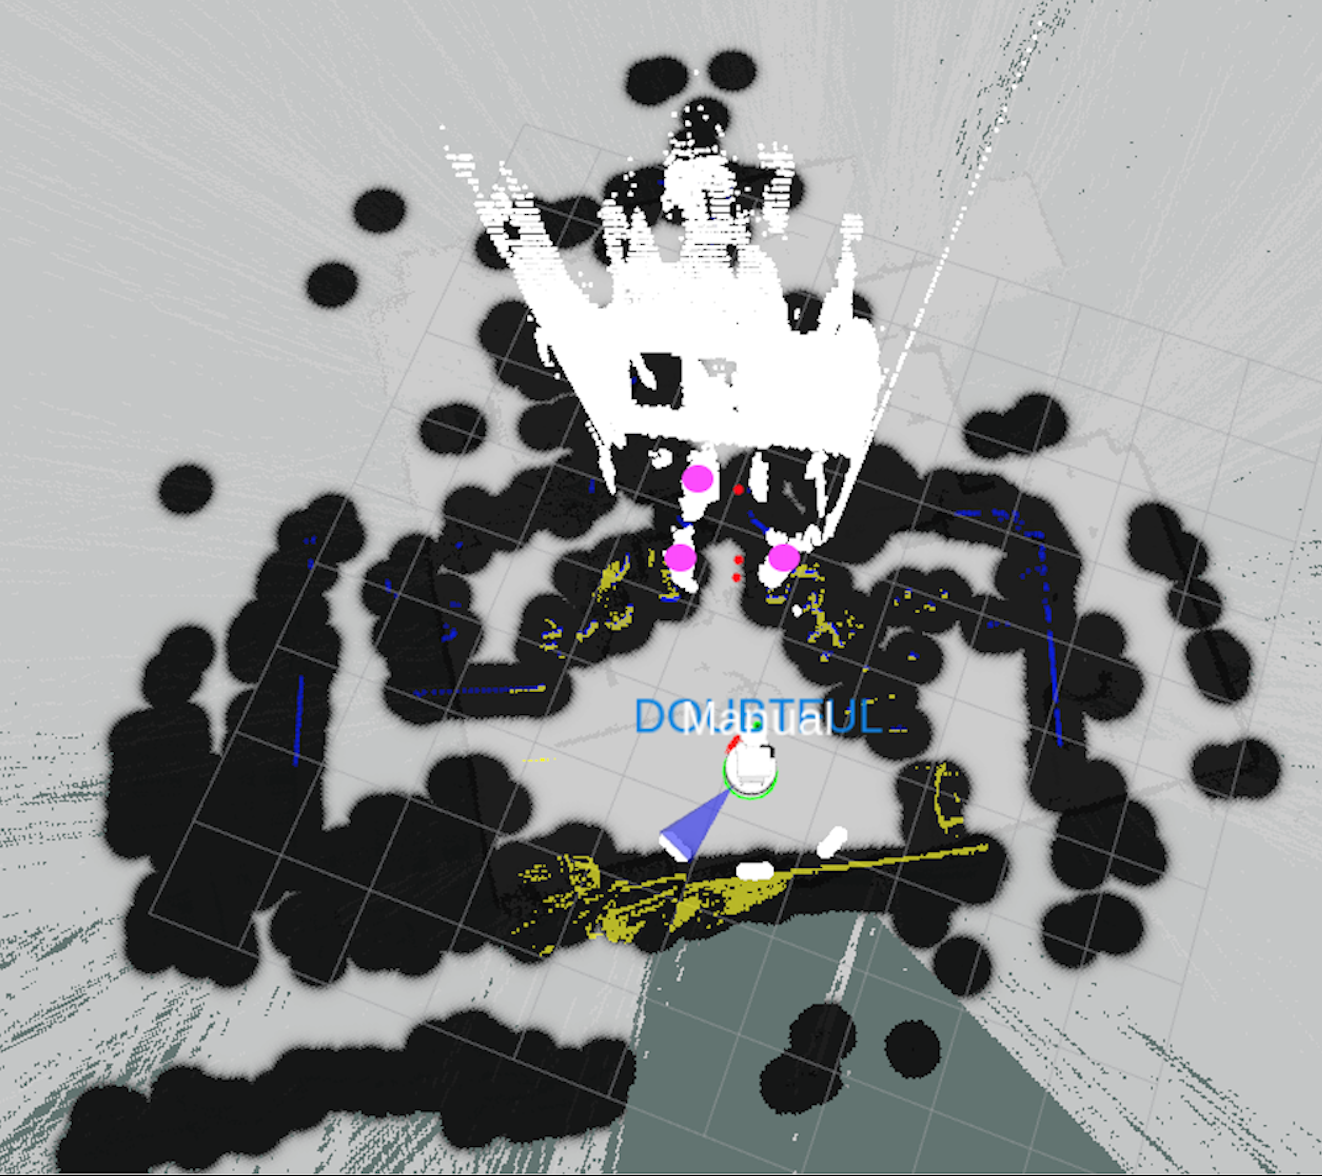
\includegraphics[width=.9\linewidth]{images/chapter6_extend3.png}
        \caption{Scenario1 markers.}
        \label{2b}
	\end{subfigure}
\end{figure}

\begin{table}[H]
  \centering
  \begin{tabular}{ |p{4cm}|p{2cm}|p{2cm}|p{2cm}|  }
    \hline
    \multicolumn{4}{|c|}{Scenario1: 3D Pose Data} \\
    \hline
    & \textbf{X} & \textbf{Y} & \textbf{Z} \\
    \hline
    Real (Left) & 1.33 & 0.0972 & 0.00441 \\
    Estimated (Left) & 1.21 & 0.124 & 0.00203 \\
    \hline
    Real (Centre) & 0.0497 & 0.264 & 0.00149 \\
    Estimated (Centre) & 0.283 & 0.344 & 0.00475 \\
    \hline
    Real(Right) & 0.0497 & 0.264 & 0.00149 \\
    Estimated(Right) & 0.283 & 0.344 & 0.00475 \\
    \hline
  \end{tabular}
\end{table}
